% Options for packages loaded elsewhere
\PassOptionsToPackage{unicode}{hyperref}
\PassOptionsToPackage{hyphens}{url}
%
\documentclass[
]{article}
\usepackage{amsmath,amssymb}
\usepackage{lmodern}
\usepackage{ifxetex,ifluatex}
\ifnum 0\ifxetex 1\fi\ifluatex 1\fi=0 % if pdftex
  \usepackage[T1]{fontenc}
  \usepackage[utf8]{inputenc}
  \usepackage{textcomp} % provide euro and other symbols
\else % if luatex or xetex
  \usepackage{unicode-math}
  \defaultfontfeatures{Scale=MatchLowercase}
  \defaultfontfeatures[\rmfamily]{Ligatures=TeX,Scale=1}
\fi
% Use upquote if available, for straight quotes in verbatim environments
\IfFileExists{upquote.sty}{\usepackage{upquote}}{}
\IfFileExists{microtype.sty}{% use microtype if available
  \usepackage[]{microtype}
  \UseMicrotypeSet[protrusion]{basicmath} % disable protrusion for tt fonts
}{}
\makeatletter
\@ifundefined{KOMAClassName}{% if non-KOMA class
  \IfFileExists{parskip.sty}{%
    \usepackage{parskip}
  }{% else
    \setlength{\parindent}{0pt}
    \setlength{\parskip}{6pt plus 2pt minus 1pt}}
}{% if KOMA class
  \KOMAoptions{parskip=half}}
\makeatother
\usepackage{xcolor}
\IfFileExists{xurl.sty}{\usepackage{xurl}}{} % add URL line breaks if available
\IfFileExists{bookmark.sty}{\usepackage{bookmark}}{\usepackage{hyperref}}
\hypersetup{
  pdftitle={MovieLens Recommendation System - Report},
  pdfauthor={Uday Adusumilli},
  hidelinks,
  pdfcreator={LaTeX via pandoc}}
\urlstyle{same} % disable monospaced font for URLs
\usepackage[margin=1in]{geometry}
\usepackage{graphicx}
\makeatletter
\def\maxwidth{\ifdim\Gin@nat@width>\linewidth\linewidth\else\Gin@nat@width\fi}
\def\maxheight{\ifdim\Gin@nat@height>\textheight\textheight\else\Gin@nat@height\fi}
\makeatother
% Scale images if necessary, so that they will not overflow the page
% margins by default, and it is still possible to overwrite the defaults
% using explicit options in \includegraphics[width, height, ...]{}
\setkeys{Gin}{width=\maxwidth,height=\maxheight,keepaspectratio}
% Set default figure placement to htbp
\makeatletter
\def\fps@figure{htbp}
\makeatother
\setlength{\emergencystretch}{3em} % prevent overfull lines
\providecommand{\tightlist}{%
  \setlength{\itemsep}{0pt}\setlength{\parskip}{0pt}}
\setcounter{secnumdepth}{5}
\usepackage{booktabs}
\usepackage{longtable}
\usepackage{array}
\usepackage{multirow}
\usepackage{wrapfig}
\usepackage{float}
\usepackage{colortbl}
\usepackage{pdflscape}
\usepackage{tabu}
\usepackage{threeparttable}
\usepackage{threeparttablex}
\usepackage[normalem]{ulem}
\usepackage{makecell}
\usepackage{xcolor}
\ifluatex
  \usepackage{selnolig}  % disable illegal ligatures
\fi

\title{MovieLens Recommendation System - Report}
\author{Uday Adusumilli}
\date{18 February, 2022}

\begin{document}
\maketitle

{
\setcounter{tocdepth}{2}
\tableofcontents
}
\newpage

\hypertarget{executive-summary}{%
\section{Executive Summary}\label{executive-summary}}

The purpose for this project is creating a recommender system using
MovieLens dataset.

The version of movielens dataset used for this final assignment contains
approximately 10 Milions of movies ratings, divided in 9 Milions for
training and one Milion for validation. It is a small subset of a much
larger (and famous) dataset with several millions of ratings. Into the
training dataset there are approximately \textbf{70.000 users} and
\textbf{11.000 different movies} divided in 20 genres such as Action,
Adventure, Horror, Drama, Thriller and more.

After a initial data exploration, the recommender systems builted on
this dataset are evaluated and choosen based on the RMSE - Root Mean
Squared Error that should be at least lower than \textbf{0.87750}.

\[\mbox{RMSE} = \sqrt{\frac{1}{n}\sum_{t=1}^{n}e_t^2}\]

For accomplishing this goal, the \textbf{Regularized Movie+User+Genre
Model} is capable to reach a RMSE of \textbf{0.8628}, that is really
good.

\hypertarget{exploratory-data-analysis}{%
\section{Exploratory Data Analysis}\label{exploratory-data-analysis}}

\hypertarget{inital-data-exploration}{%
\subsection{Inital data Exploration}\label{inital-data-exploration}}

The 10 Millions dataset is divided into two dataset: \texttt{edx} for
training purpose and \texttt{validation} for the validation phase.

The \texttt{edx} dataset contains approximately 9 Millions of rows with
70.000 different users and 11.000 movies with rating score between 0.5
and 5. There is no missing values (0 or NA).

\textbf{edx dataset}

\begin{table}
\centering\begingroup\fontsize{10}{12}\selectfont

\begin{tabular}{r|r}
\hline
Users & Movies\\
\hline
69878 & 10677\\
\hline
\end{tabular}
\endgroup{}
\end{table}

\textbf{Missing Values per Column}

\begin{table}
\centering\begingroup\fontsize{10}{12}\selectfont

\begin{tabular}{l|r}
\hline
  & x\\
\hline
userId & 0\\
\hline
movieId & 0\\
\hline
rating & 0\\
\hline
timestamp & 0\\
\hline
title & 0\\
\hline
genres & 0\\
\hline
\end{tabular}
\endgroup{}
\end{table}

The features/variables/columns in both datasets are six:

\begin{itemize}
\tightlist
\item
  \textbf{userId} \texttt{\textless{}integer\textgreater{}} that
  contains the unique identification number for each user.
\item
  \textbf{movieId} \texttt{\textless{}numeric\textgreater{}} that
  contains the unique identification number for each movie.
\item
  \textbf{rating} \texttt{\textless{}numeric\textgreater{}} that
  contains the rating of one movie by one user. Ratings are made on a
  5-Star scale with half-star increments.
\item
  \textbf{timestamp} \texttt{\textless{}integer\textgreater{}} that
  contains the timestamp for one specific rating provided by one user.
\item
  \textbf{title} \texttt{\textless{}character\textgreater{}} that
  contains the title of each movie including the year of the release.
\item
  \textbf{genres} \texttt{\textless{}character\textgreater{}} that
  contains a list of pipe-separated of genre of each movie.
\end{itemize}

\newpage

\textbf{First 6 Rows of edx dataset}

\begin{table}
\centering\begingroup\fontsize{10}{12}\selectfont

\begin{tabular}{r|r|r|r|l|l}
\hline
userId & movieId & rating & timestamp & title & genres\\
\hline
1 & 122 & 5 & 838985046 & Boomerang (1992) & Comedy|Romance\\
\hline
1 & 185 & 5 & 838983525 & Net, The (1995) & Action|Crime|Thriller\\
\hline
1 & 231 & 5 & 838983392 & Dumb \& Dumber (1994) & Comedy\\
\hline
1 & 292 & 5 & 838983421 & Outbreak (1995) & Action|Drama|Sci-Fi|Thriller\\
\hline
1 & 316 & 5 & 838983392 & Stargate (1994) & Action|Adventure|Sci-Fi\\
\hline
1 & 329 & 5 & 838983392 & Star Trek: Generations (1994) & Action|Adventure|Drama|Sci-Fi\\
\hline
\end{tabular}
\endgroup{}
\end{table}

\hypertarget{dataset-pre-processing-and-feature-engineering}{%
\subsection{Dataset Pre-Processing and Feature
Engineering}\label{dataset-pre-processing-and-feature-engineering}}

After a initial data exploration, we notice that the \texttt{genres} are
pipe-separated values. It's necessary to extract them for more
consisten, robust and precise estimate. We also observe that the
\texttt{title} contains the year where the movie war released and this
it could be necessary to predic the movie rating. Finally, we can
extract the year and the month for each rating.

The pre-processing phase is composed by this steps:

\begin{enumerate}
\def\labelenumi{\arabic{enumi}.}
\tightlist
\item
  Convert \texttt{timestamp} to a human readable date format;
\item
  Extract the month and the year from the date;
\item
  Extract the release year for each movie from the title;
\item
  Separate each genre from the pipe-separated value. It increases the
  size of both datasets.
\end{enumerate}

After preprocessing the data, \texttt{edx} dataset looks like this:

\textbf{Processed edx datadaset}

\begin{table}
\centering\begingroup\fontsize{10}{12}\selectfont

\begin{tabular}{r|r|r|l|l|r|r|r}
\hline
userId & movieId & rating & title & genre & release & yearOfRate & monthOfRate\\
\hline
1 & 122 & 5 & Boomerang & Comedy & 1992 & 1996 & 8\\
\hline
1 & 122 & 5 & Boomerang & Romance & 1992 & 1996 & 8\\
\hline
1 & 185 & 5 & Net, The & Action & 1995 & 1996 & 8\\
\hline
1 & 185 & 5 & Net, The & Crime & 1995 & 1996 & 8\\
\hline
1 & 185 & 5 & Net, The & Thriller & 1995 & 1996 & 8\\
\hline
1 & 231 & 5 & Dumb \& Dumber & Comedy & 1994 & 1996 & 8\\
\hline
\end{tabular}
\endgroup{}
\end{table}

\newpage

\hypertarget{rating-distribution}{%
\subsection{Rating Distribution}\label{rating-distribution}}

\textbf{Overview of Rating Distribution}

According to the histogram below, it shows that there are a small amount
of negative votes (below 3). Maybe, the user tends to give a vote if he
liked the movie. Half-Star votes are less common than ``Full-Star''
votes.

\begin{center}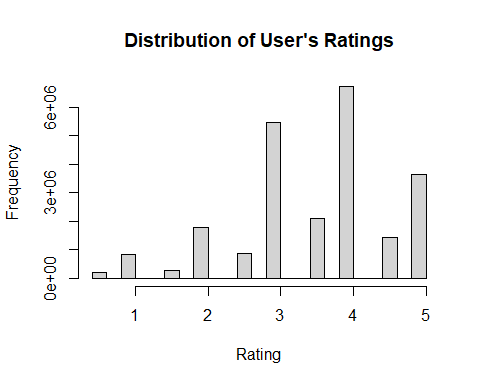
\includegraphics{MovieLens-Project-Report_files/figure-latex/unnamed-chunk-16-1} \end{center}

\textbf{Overview of Rating Frequency through Months and Years}

\begin{center}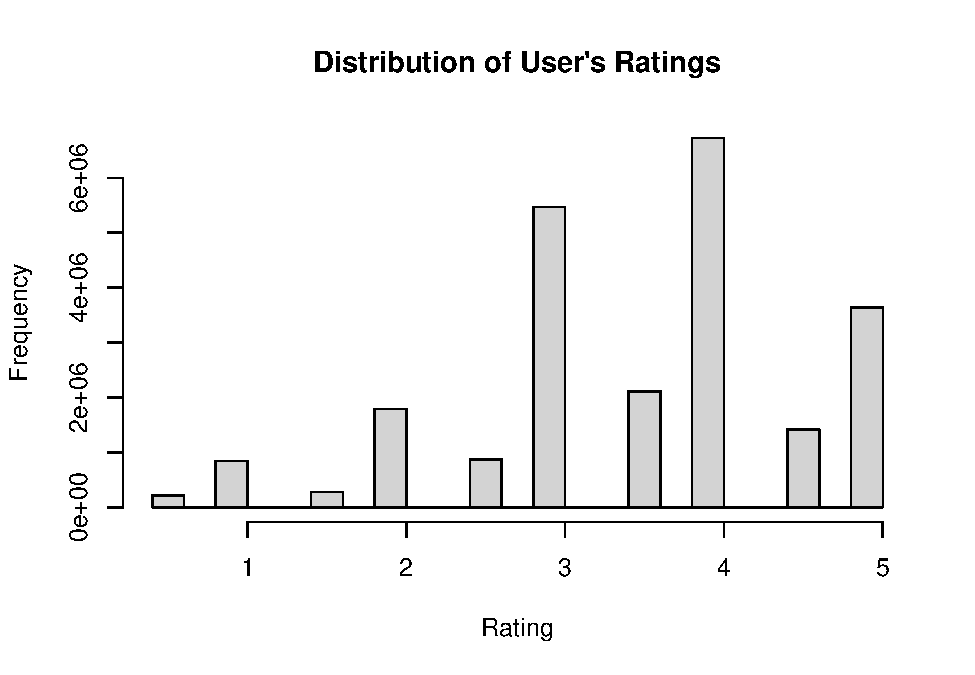
\includegraphics{MovieLens-Project-Report_files/figure-latex/unnamed-chunk-17-1} \end{center}

\begin{center}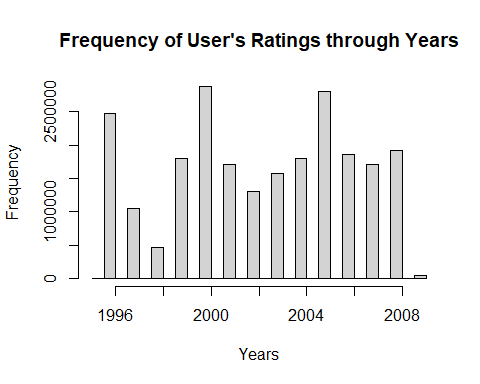
\includegraphics{MovieLens-Project-Report_files/figure-latex/unnamed-chunk-17-2} \end{center}

\hypertarget{numbers-of-ratings-per-movie}{%
\subsubsection{Numbers of Ratings per
Movie}\label{numbers-of-ratings-per-movie}}

\begin{center}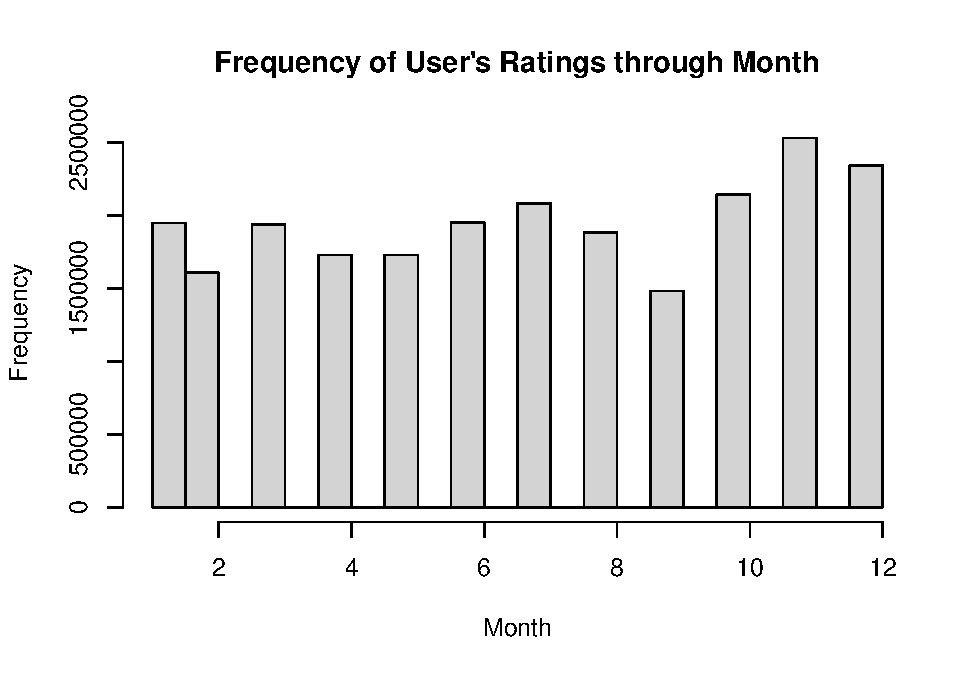
\includegraphics{MovieLens-Project-Report_files/figure-latex/unnamed-chunk-18-1} \end{center}

\hypertarget{top-rated-movies}{%
\subsubsection{Top Rated Movies}\label{top-rated-movies}}

\begin{center}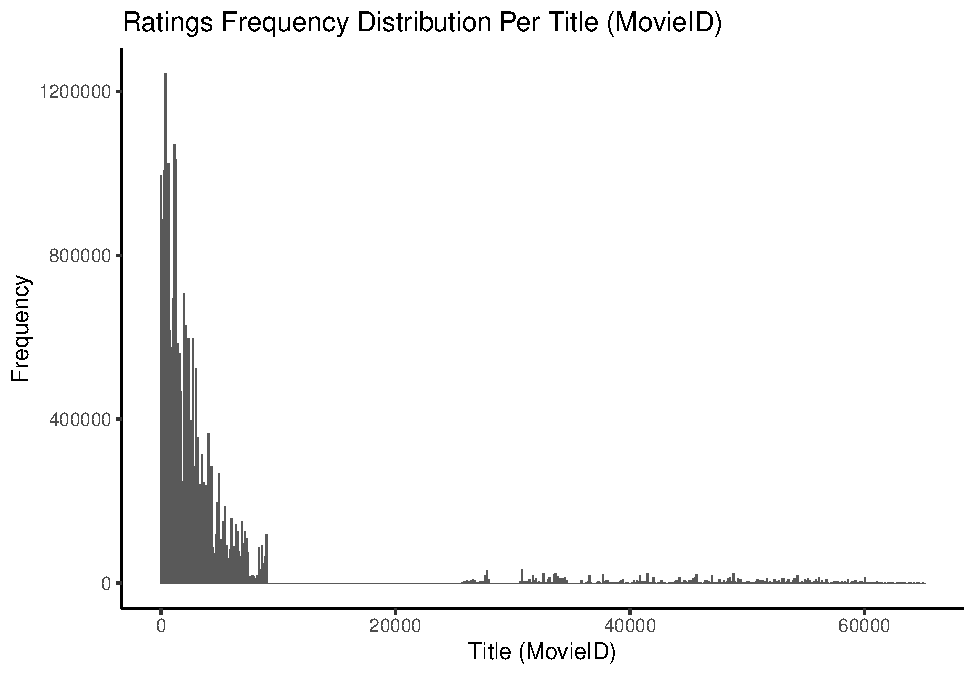
\includegraphics{MovieLens-Project-Report_files/figure-latex/unnamed-chunk-19-1} \end{center}

\begin{table}
\centering\begingroup\fontsize{10}{12}\selectfont

\begin{tabular}{l|r}
\hline
title & count\\
\hline
Forrest Gump & 124304\\
\hline
Toy Story & 119130\\
\hline
Jurassic Park & 117164\\
\hline
True Lies & 113930\\
\hline
Aladdin & 106070\\
\hline
Batman & 98656\\
\hline
Lion King, The & 94435\\
\hline
Pulp Fiction & 94008\\
\hline
Independence Day (a.k.a. ID4) & 93440\\
\hline
Silence of the Lambs, The & 90840\\
\hline
Beauty and the Beast & 89315\\
\hline
Fargo & 85480\\
\hline
Seven (a.k.a. Se7en) & 81084\\
\hline
Braveheart & 78774\\
\hline
Shrek & 78564\\
\hline
Star Wars: Episode IV - A New Hope (a.k.a. Star Wars) & 77427\\
\hline
Ghost & 77335\\
\hline
Who Framed Roger Rabbit? & 76825\\
\hline
Mission: Impossible & 75876\\
\hline
Princess Bride, The & 74045\\
\hline
Dances with Wolves & 69936\\
\hline
Blade Runner & 69615\\
\hline
Batman Forever & 69432\\
\hline
Mask, The & 68200\\
\hline
Babe & 68140\\
\hline
\end{tabular}
\endgroup{}
\end{table}

\hypertarget{mean-distribution-per-title-movie-id}{%
\subsubsection{Mean Distribution per Title (Movie
ID)}\label{mean-distribution-per-title-movie-id}}

\begin{center}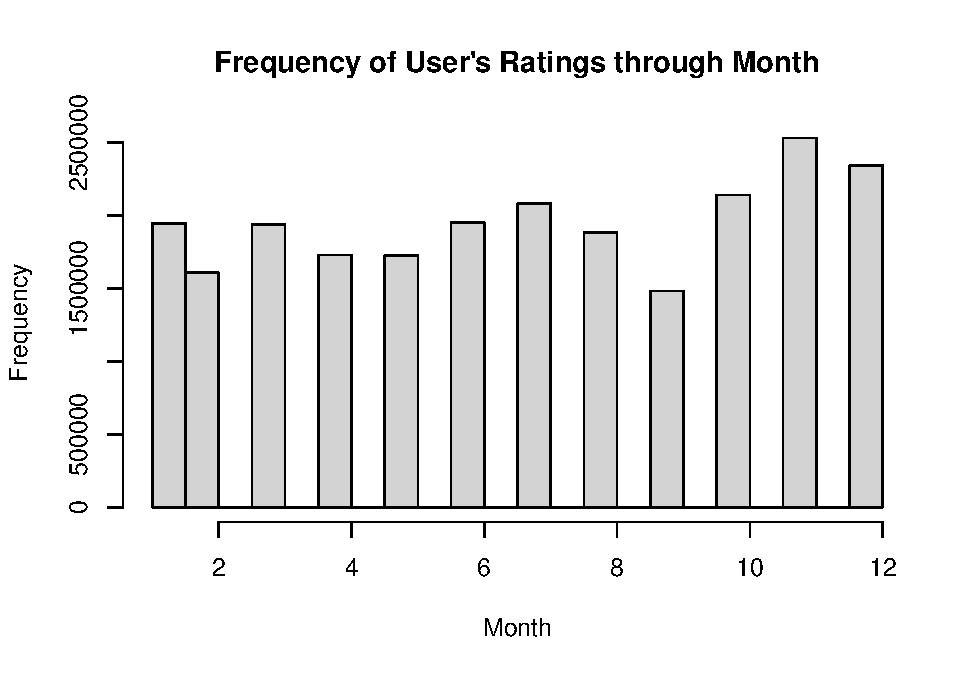
\includegraphics{MovieLens-Project-Report_files/figure-latex/unnamed-chunk-21-1} \end{center}

\begin{table}
\centering\begingroup\fontsize{10}{12}\selectfont

\begin{tabular}{l|r}
\hline
title & mean\\
\hline
Blue Light, The (Das Blaue Licht) & 5.000000\\
\hline
Constantine's Sword & 5.000000\\
\hline
Fighting Elegy (Kenka erejii) & 5.000000\\
\hline
Hellhounds on My Trail & 5.000000\\
\hline
Satan's Tango (Sátántangó) & 5.000000\\
\hline
Shadows of Forgotten Ancestors & 5.000000\\
\hline
Sun Alley (Sonnenallee) & 5.000000\\
\hline
Human Condition II, The (Ningen no joken II) & 4.833333\\
\hline
Human Condition III, The (Ningen no joken III) & 4.750000\\
\hline
Who's Singin' Over There? (a.k.a. Who Sings Over There) (Ko to tamo peva) & 4.750000\\
\hline
Class, The (Entre les Murs) & 4.666667\\
\hline
I'm Starting From Three (Ricomincio da Tre) & 4.666667\\
\hline
Man Who Planted Trees, The (Homme qui plantait des arbres, L') & 4.571429\\
\hline
Bad Blood (Mauvais sang) & 4.500000\\
\hline
Caótica Ana & 4.500000\\
\hline
Demon Lover Diary & 4.500000\\
\hline
End of Summer, The (Kohayagawa-ke no aki) & 4.500000\\
\hline
Fires on the Plain (Nobi) & 4.500000\\
\hline
Ladrones & 4.500000\\
\hline
Life of Oharu, The (Saikaku ichidai onna) & 4.500000\\
\hline
Man Named Pearl, A & 4.500000\\
\hline
Mickey & 4.500000\\
\hline
Please Vote for Me & 4.500000\\
\hline
Power of Nightmares: The Rise of the Politics of Fear, The & 4.500000\\
\hline
Testament of Orpheus, The (Testament d'Orphée) & 4.500000\\
\hline
\end{tabular}
\endgroup{}
\end{table}

\hypertarget{median-distribution-per-title-movie-id}{%
\subsubsection{Median Distribution per Title (Movie
ID)}\label{median-distribution-per-title-movie-id}}

\begin{center}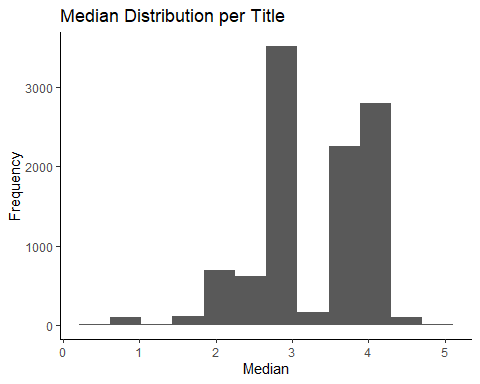
\includegraphics{MovieLens-Project-Report_files/figure-latex/unnamed-chunk-23-1} \end{center}

\begin{table}
\centering\begingroup\fontsize{10}{12}\selectfont

\begin{tabular}{l|r}
\hline
title & median\\
\hline
Aerial, The (La Antena) & 5.00\\
\hline
Blue Light, The (Das Blaue Licht) & 5.00\\
\hline
Class, The (Entre les Murs) & 5.00\\
\hline
Constantine's Sword & 5.00\\
\hline
Fighting Elegy (Kenka erejii) & 5.00\\
\hline
Godfather, The & 5.00\\
\hline
Hellhounds on My Trail & 5.00\\
\hline
Human Condition II, The (Ningen no joken II) & 5.00\\
\hline
Jesus & 5.00\\
\hline
Kids of Survival & 5.00\\
\hline
Man Who Planted Trees, The (Homme qui plantait des arbres, L') & 5.00\\
\hline
Parallel Sons & 5.00\\
\hline
Satan's Tango (Sátántangó) & 5.00\\
\hline
Shadows of Forgotten Ancestors & 5.00\\
\hline
Shawshank Redemption, The & 5.00\\
\hline
Sun Alley (Sonnenallee) & 5.00\\
\hline
Who's Singin' Over There? (a.k.a. Who Sings Over There) (Ko to tamo peva) & 5.00\\
\hline
World of Apu, The (Apur Sansar) & 5.00\\
\hline
Human Condition III, The (Ningen no joken III) & 4.75\\
\hline
400 Blows, The (Les Quatre cents coups) & 4.50\\
\hline
49 Up & 4.50\\
\hline
Amelie (Fabuleux destin d'Amélie Poulain, Le) & 4.50\\
\hline
American Beauty & 4.50\\
\hline
Andrei Rublev (Andrey Rublyov) & 4.50\\
\hline
Bad Blood (Mauvais sang) & 4.50\\
\hline
\end{tabular}
\endgroup{}
\end{table}

\hypertarget{genre-analysis}{%
\subsection{Genre Analysis}\label{genre-analysis}}

\hypertarget{rating-distribution-per-genre}{%
\subsubsection{Rating Distribution per
Genre}\label{rating-distribution-per-genre}}

\textbf{Overview of Rating distribution over Genre}

\begin{center}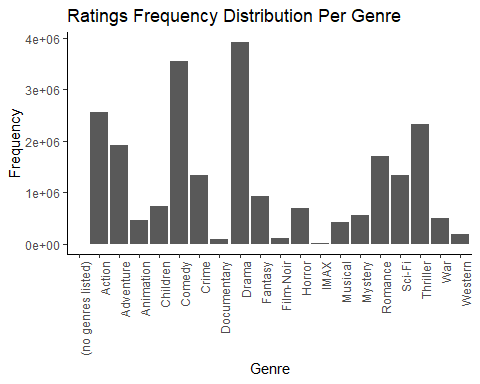
\includegraphics{MovieLens-Project-Report_files/figure-latex/unnamed-chunk-25-1} \end{center}

\begin{table}
\centering\begingroup\fontsize{10}{12}\selectfont

\begin{tabular}{l|r}
\hline
genre & count\\
\hline
Drama & 3909401\\
\hline
Comedy & 3541284\\
\hline
Action & 2560649\\
\hline
Thriller & 2325349\\
\hline
Adventure & 1908692\\
\hline
Romance & 1712232\\
\hline
Sci-Fi & 1341750\\
\hline
Crime & 1326917\\
\hline
Fantasy & 925624\\
\hline
Children & 737851\\
\hline
Horror & 691407\\
\hline
Mystery & 567865\\
\hline
War & 511330\\
\hline
Animation & 467220\\
\hline
Musical & 432960\\
\hline
Western & 189234\\
\hline
Film-Noir & 118394\\
\hline
Documentary & 93252\\
\hline
IMAX & 8190\\
\hline
(no genres listed) & 6\\
\hline
\end{tabular}
\endgroup{}
\end{table}

\hypertarget{mean-distribution-per-genre}{%
\subsubsection{Mean Distribution per
Genre}\label{mean-distribution-per-genre}}

\begin{center}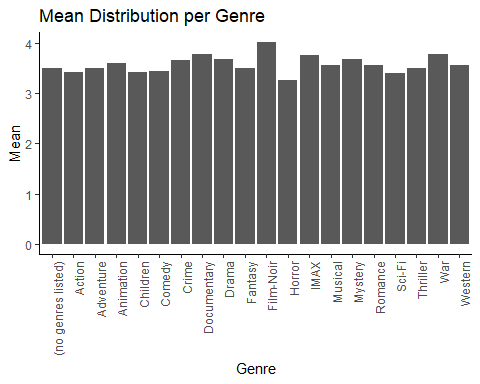
\includegraphics{MovieLens-Project-Report_files/figure-latex/unnamed-chunk-27-1} \end{center}

\begin{table}
\centering\begingroup\fontsize{10}{12}\selectfont

\begin{tabular}{l|r}
\hline
genre & mean\\
\hline
Film-Noir & 4.011732\\
\hline
Documentary & 3.784385\\
\hline
War & 3.779457\\
\hline
IMAX & 3.761844\\
\hline
Mystery & 3.677412\\
\hline
Drama & 3.673047\\
\hline
Crime & 3.666151\\
\hline
Animation & 3.599588\\
\hline
Musical & 3.562761\\
\hline
Western & 3.555122\\
\hline
Romance & 3.553594\\
\hline
Thriller & 3.506879\\
\hline
Fantasy & 3.502419\\
\hline
(no genres listed) & 3.500000\\
\hline
Adventure & 3.494076\\
\hline
Comedy & 3.437040\\
\hline
Action & 3.421589\\
\hline
Children & 3.418673\\
\hline
Sci-Fi & 3.396756\\
\hline
Horror & 3.269523\\
\hline
\end{tabular}
\endgroup{}
\end{table}

\hypertarget{median-distribution-per-genre}{%
\subsubsection{Median Distribution per
Genre}\label{median-distribution-per-genre}}

\begin{center}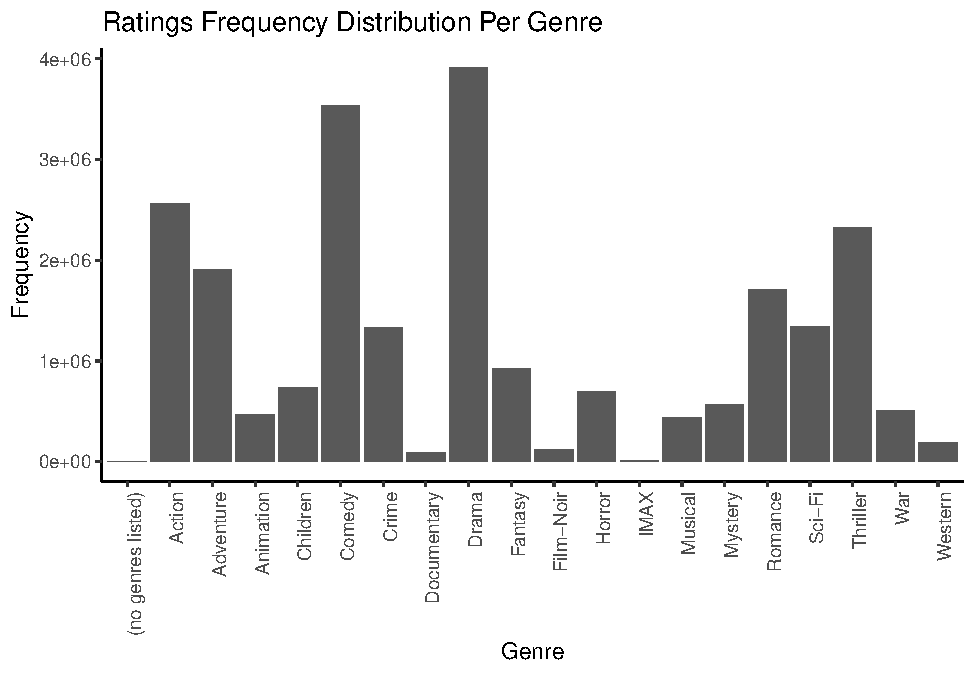
\includegraphics{MovieLens-Project-Report_files/figure-latex/unnamed-chunk-29-1} \end{center}

\begin{table}
\centering\begingroup\fontsize{10}{12}\selectfont

\begin{tabular}{l|r}
\hline
genre & median\\
\hline
Animation & 4.0\\
\hline
Crime & 4.0\\
\hline
Documentary & 4.0\\
\hline
Drama & 4.0\\
\hline
Film-Noir & 4.0\\
\hline
IMAX & 4.0\\
\hline
Musical & 4.0\\
\hline
Mystery & 4.0\\
\hline
Romance & 4.0\\
\hline
War & 4.0\\
\hline
Western & 4.0\\
\hline
(no genres listed) & 3.5\\
\hline
Action & 3.5\\
\hline
Adventure & 3.5\\
\hline
Children & 3.5\\
\hline
Comedy & 3.5\\
\hline
Fantasy & 3.5\\
\hline
Horror & 3.5\\
\hline
Sci-Fi & 3.5\\
\hline
Thriller & 3.5\\
\hline
\end{tabular}
\endgroup{}
\end{table}

\hypertarget{analysis---model-building-and-evaluation}{%
\section{Analysis - Model Building and
Evaluation}\label{analysis---model-building-and-evaluation}}

\hypertarget{naive-baseline-model}{%
\subsection{Naive Baseline Model}\label{naive-baseline-model}}

The simplest model that someone can build, is a Naive Model that predict
ALWAYS the mean. In this case, the mean is approximately 3.5.

\begin{verbatim}
## [1] "The mean is: 3.52700364195256"
\end{verbatim}

\hypertarget{naive-mean-baseline-model}{%
\subsubsection{Naive Mean-Baseline
Model}\label{naive-mean-baseline-model}}

The formula used is:

\[Y_{u,i} = \hat{\mu} + \varepsilon_{u,i}\]

With \(\hat{\mu}\) is the mean and \(\varepsilon_{i,u}\) is the
independent errors sampled from the same distribution centered at 0.

The RMSE on the \texttt{validation} dataset is \textbf{1.05}. It is very
far for the target RMSE (below 0.87) and that indicates poor performance
for the model.

\hypertarget{movie-based-model-a-content-based-approach}{%
\subsection{Movie-Based Model, a Content-based
Approach}\label{movie-based-model-a-content-based-approach}}

The first Non-Naive Model takes into account the content. In this case
the movies that are rated higher or lower resperct to each other.

The formula used is:

\[Y_{u,i} = \hat{\mu} + b_i + \epsilon_{u,i}\]

With \(\hat{\mu}\) is the mean and \(\varepsilon_{i,u}\) is the
independent errors sampled from the same distribution centered at 0. The
\(b_i\) is a measure for the popularity of movie \(i\), i.e.~the bias of
movie \(i\).

The RMSE on the \texttt{validation} dataset is \textbf{0.94}. It better
than the Naive Mean-Baseline Model, but it is also very far from the
target RMSE (below 0.87) and that indicates poor performance for the
model.

\hypertarget{movie-user-model-a-user-based-approach}{%
\subsection{Movie + User Model, a User-based
approach}\label{movie-user-model-a-user-based-approach}}

The second Non-Naive Model consider that the users have different tastes
and rate differently.

The formula used is:

\[Y_{u,i} = \hat{\mu} + b_i + b_u + \epsilon_{u,i}\]

With \(\hat{\mu}\) is the mean and \(\varepsilon_{i,u}\) is the
independent errors sampled from the same distribution centered at 0. The
\(b_i\) is a measure for the popularity of movie \(i\), i.e.~the bias of
movie \(i\). The \(b_u\) is a measure for the mildness of user \(u\),
i.e.~the bias of user \(u\).

The RMSE on the \texttt{validation} dataset is \textbf{0.8635} and this
is very good. The Movie+User Based Model reaches the desidered
performance but applying the regularization techniques, can improve the
performance just a little.

\hypertarget{movie-user-genre-model-the-genre-popularity}{%
\subsection{Movie + User + Genre Model, the Genre
Popularity}\label{movie-user-genre-model-the-genre-popularity}}

The formula used is:

\[Y_{u,i} = \hat{\mu} + b_i + b_u + b_{u,g} + \epsilon_{u,i}\]

With \(\hat{\mu}\) is the mean and \(\varepsilon_{i,u}\) is the
independent errors sampled from the same distribution centered at 0. The
\(b_i\) is a measure for the popularity of movie \(i\), i.e.~the bias of
movie \(i\). The \(b_u\) is a measure for the mildness of user \(u\),
i.e.~the bias of user \(u\). The \(b_{u,g}\) is a measure for how much a
user \(u\) likes the genre \(g\).

The RMSE on the \texttt{validation} dataset is \textbf{0.8634} and this
is very good. The Movie+User+Genre Based Model reaches the desidered
performance but adding the \texttt{genre} predictor, doesn't improve
significantly the model's performance. Applying the regularization
techniques, can improve the performance just a little.

\hypertarget{regularization}{%
\subsection{Regularization}\label{regularization}}

The regularization method allows us to add a penalty \(\lambda\)
(lambda) to penalizes movies with large estimates from a small sample
size. In order to optimize \(b_i\), it necessary to use this equation:

\[\frac{1}{N} \sum_{u,i} (y_{u,i} - \mu - b_{i})^{2} + \lambda \sum_{i} b_{i}^2\]

reduced to this equation:

\[\hat{b_{i}} (\lambda) = \frac{1}{\lambda + n_{i}} \sum_{u=1}^{n_{i}} (Y_{u,i} - \hat{\mu}) \]

\hypertarget{regularized-movie-based-model}{%
\subsubsection{Regularized Movie-Based
Model}\label{regularized-movie-based-model}}

\begin{center}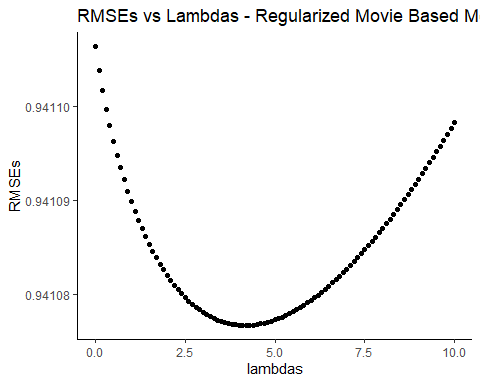
\includegraphics{MovieLens-Project-Report_files/figure-latex/unnamed-chunk-36-1} \end{center}

The RMSE on the \texttt{validation} dataset is \textbf{0.8635} and this
is very good. The Movie+User Based Model reaches the desidered
performance but applying the regularization techniques, can improve the
performance just a little.

\hypertarget{regularized-movieuser-model}{%
\subsubsection{Regularized Movie+User
Model}\label{regularized-movieuser-model}}

\begin{center}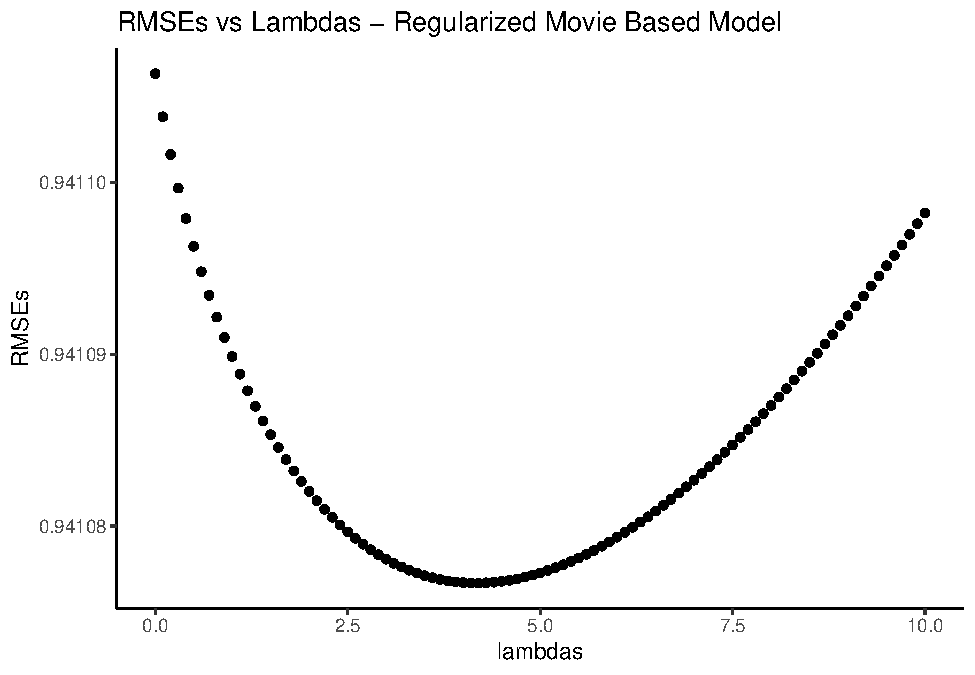
\includegraphics{MovieLens-Project-Report_files/figure-latex/unnamed-chunk-37-1} \end{center}

The RMSE on the \texttt{validation} dataset is \textbf{0.8629}. The
Regularized Movie+User Based Model improves just a little the result of
the Non-Regularized Model.

\hypertarget{regularized-movieusergenre-model}{%
\subsubsection{Regularized Movie+User+Genre
Model}\label{regularized-movieusergenre-model}}

\begin{center}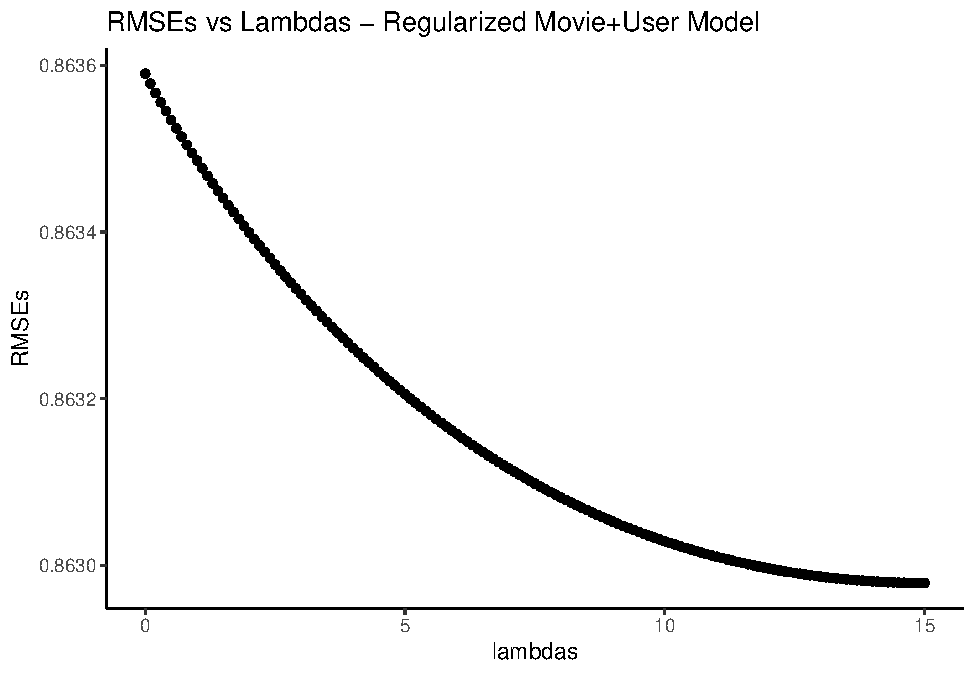
\includegraphics{MovieLens-Project-Report_files/figure-latex/unnamed-chunk-38-1} \end{center}

The RMSE on the \texttt{validation} dataset is \textbf{0.8628} and this
is the best result of the builted models. The Regularized
Movie+User+Genre Based Model improves just a little the result of the
Non-Regularized Model. As the Non-Regularized Model, the \texttt{genre}
predictor doesn't improve significantly the model's performance.

\hypertarget{results}{%
\section{Results}\label{results}}

This is the summary results for all the model builted, trained on
\texttt{edx} dataset and validated on the \texttt{validation} dataset.

\begin{table}
\centering\begingroup\fontsize{10}{12}\selectfont

\begin{tabular}{l|r}
\hline
model & RMSE\\
\hline
Naive Mean-Baseline Model & 1.0524433\\
\hline
Movie-Based Model & 0.9411063\\
\hline
Movie+User Based Model & 0.8635899\\
\hline
Movie+User+Genre Based Model & 0.8634946\\
\hline
Regularized Movie-Based Model & 0.9410767\\
\hline
Regularized Movie+User Based Model & 0.8629791\\
\hline
Regularized Movie+User+Genre Based Model & 0.8628874\\
\hline
\end{tabular}
\endgroup{}
\end{table}

\hypertarget{conclusion}{%
\section{Conclusion}\label{conclusion}}

After training different models, it's very clear that \texttt{movieId}
and \texttt{userId} contribute more than the \texttt{genre} predictor.
Without regularization, the model can archieves and overtakes the
desidered peformance, but the best is the enemy of the good and applying
regularization and adding the \texttt{genre} predictor, it make possible
to reach a RSME of \textbf{0.8628} that is the best result for the
trained models.

\end{document}
